\documentclass[a4paper]{article}

\usepackage{authblk}
\usepackage[ruled,algosection,noend,linesnumbered]{algorithm2e}
\usepackage{amsmath}
\usepackage{amsthm}
\usepackage{amsfonts}
\usepackage{subcaption}
\usepackage{tikz}
\usepackage{cite}
\usetikzlibrary{calc, automata, chains}

\newtheorem{privdef}{Privacy Definition}
\newtheorem{secthm}{Security Theorem}

\newcommand{\raphael}[1]{\textcolor{blue}{Raphael: #1}}
\newcommand{\george}[1]{\textcolor{green}{George: #1}}

\begin{document}

\author{Raphael R. Toledo \thanks{E-mail: r.toledo@cs.ucl.ac.uk} }
\author{George Danezis \thanks{E-mail: g.danezis@cs.ucl.ac.uk} }

\affil{University College London }

\title{Oblivious RAM: towards a shuffle amortization.}
%what matters the most ? The sorting algo or the use of mixnets ?

\maketitle

\begin{abstract}
{
We present in this paper an ORAM system relying on mixnet technologies for the eviction process.
}
\end{abstract}

\section{Introduction}
Cloud technologies provide a range of services using remote servers, including website hosting, computation, and data storage. One of the main issues for the providers is to protect the users, not only against active adversaries, who resolutely hinder a user, but also against passive ones, and doing so for reasonable costs. 
Cryptographic functions are thus used among other things to create secure communication channels, authenticate users, encrypt and check the data integrity. These solutions however do not prevent the leakage of some information and its interception : an adversary can count the number of packets exchanged by two parties, even when using anonymity systems \cite{murdoch2005}, and guess which file was accessed thanks to a-priori knowledge : the file size distribution, the file access frequency distribution, etc..
Oblivious RAM (ORAM)~\cite{goldreich87}, or Oblivious Storage (OS)~\cite{boneh2011}, are key technologies to answer such problem by hiding the pattern access.\\

Most of existing ORAM solutions so far have required the whole database to be periodically rerandomized by the user. Improvements have been made on the eviction process thanks to structural change in the data representation, considering trees or rings, and the shuffling algorithm, in particular with the introduction of dummies.
In 2013, Stefanov and Shi~\cite{stefanov2013} proposed a multi-cloud oblivious storage where two or more semi-trusted clouds are used to serve user requests and hide the access pattern concurrently. However, the practicality of owning and managing more than a cloud was not discussed in the paper. \\

In this work, we present a new security defition relying on indistiguishability assumptions and suggest to leave the eviction and shuffling to untrusted third partys and attest its privacy thanks to an information theoric proof.
The advantages of such use are the delegation of the shuffling, the possibility to postpone the latter to quieter times and the independance to centralized parties.

\subsection{Related Work}
\subsubsection{ORAM}

\subsubsection{Mixnets.}

\subsubsection{Shuffling and Sorting.}


\noindent\textbf{Shuffling} \\

Random transpositions shuffle (RTS) have been thoroughly studied since 1981 when Diaconis and Ashahshahani released their paper on random permutation generations~cite{}.
RTS consists in randomly selecting two cards from a deck of cards and exchange them if they are different.
The time of convergence towards the uniform distribution, the mixing time, was bounded at $\left(2+o(1)\right)n\log(n)$ thanks to strong a stationary time argument due to Broder\cite{}.
Diaconis however observed a cutoff phenomenon in his first paper in 1981, an abrupt convergence to the equilibrium distribution, at $\frac{1}{2}n\log(n)$ of width $O(n)$.\\

\noindent\textbf{Sorting} \\
- sorting networks\\
- Melbourne shuffle\\

\subsection{Our contributions}

\subsection{Content}

\section{Preliminaries}
\subsection{Model}
We consider a system composed of a remote server running the ORAM protocol with storage of size O($N$) where $N$ corresponds to the number of $b$ bits cipher blocks the user owns and a mixnet of $m$ mixes.
The client includes a storage manager and a stash of $s$-block capacity. 

\subsection{Threat model}
We consider an adversary $\mathcal{A}$ has corrupted $m_{a}$ mixes and potentially the ORAM database in order to discover the relationship between the records and the indexes. 
The corrupted servers are said honest but curious in that they perform correctly the assigned protocols and algorithms but passively record and share all information they observe to achieve this objective.
We also assume that the adversary observes all the user's incoming and outgoing communication.
However, we assume that all messages, database request or mix packet, are encrypted and that only message timing, volume and size from honest servers are visible to the adversary.
Attacks and countermeasures, together with the implied costs, will only be examined in the Discussion section (c.f. Section.\cite{}).

\subsection{Costs}
This work studies PIR scalability, and we focus on analyzing costs on the server side, which is the performance bottleneck of current techniques.
We denote the communication costs by $C_d$ for the number of \emph{bits} sent by the ORAM, $C_{c}$ by the client to $\mathcal{DS}$, and by $C_{m}$ sent by the mixes. 
We will call $C_p$ the computation cost derived from the mixes' permutation and $C_a$ from the database accesses.


\section{Mix-ORAM}

Reencryption network vs Decryption network. Reencryption ORAM will be used as decryption requires the user to update all records with all the keys... (except two layer encryption?).
Symmetrical Reencryption network ?

\subsection{Operation and Messages}
\section{The Eviction process.}
\subsection{Amortizing the Eviction.}
In this section we look at transposition shuffles and their use in order to amortize over time the database randomization happening during the eviction process.
We first present the mixing time of $k$-random transposition shuffles before introducing ORAM assumptions to reduce even more the expected time to achieve randomness to the eyes of the adversary.

\subsubsection{$k$-Random Transposition Shuffle.}
%We first argue that using $k$-random transposition shuffles in both the ORAM randomization and access method could help to spread over time the shuffling of the database.
Random Transposition Shuffles (RTS) are widely used examples in card shuffling: a player selects two cards of a deck, throw a coin and permute them accordingly before putting them back at the same location.
We call an oblivious $k$-random transposition shuffle (RTS) a similar process consisting in a user fetching $k$ out of $n$ records from a remote server, permuting them locally, and uploading them at the same location.

\begin{secthm}
A $k$-permutation shuffle of a $n$ card game reaches the uniform distribution in $\tau$ rounds, such that
\begin{align*}
E(\tau) &< \frac{2}{k}\cdot\frac{n^2}{n+1}\cdot \left ( \log(n) + \mathcal{O}(1) \right ) &\\
\sigma^2(\tau) &< \frac{4}{3} \cdot {\pi}^2 \cdot \left ( \frac{n}{k} \right )^2 &\\
\tau\left (\epsilon \right ) &\geq \frac{n-1}{2k} \ln{n\cdot \frac{1-\epsilon}{6}}&
\end{align*}
\end{secthm}

A $k$-RTS thus implies computation and communication cost of the order of $\mathcal{O} \left(n\cdot \log(n)\right)$.

\subsubsection{Oblivious Merge}
Before the eviction algorithm is run, the database can be represented as a simple binary array of $n$ bits out of which $s$ are 1s and $n-s$ are 0s. These two sets respectively corresponds to records which were accessed, the 1s, ot not, the 0s, by the user.
We argue that in this representation, elements of the same sets are indistiguishable to the adversary thanks to prior encryption and permutation. This simplifing assumption significantly the number of possible orderings in the adversarial view, there now are ${n \choose s}$ arrangings instead of $n!$ (proof thanks to the Stars and Bars theorem) which represents a gain of order $\mathcal{O}\left ( (n-s)!\cdot s!\right )$.

To consider an oblivious merge of these two sets, we consider the user having a local memory of capacity $m$ fetches elements from the two sets, permutes them locally, refreshes the encryption again before uploading them back at the same locations.

\begin{secthm}
An oblivious merge of 2 indistiguishable sets of respective size $n$ and $s$ requires $\tau$ rounds such that any arranging is possible, with
\begin{align*}
\tau \leq s \ln{s}&
\end{align*}
Proof can be found in Annex.~\cite{}.
\end{secthm}

\subsubsection{Amortizable sort}

We now use the $k$-RTS and Oblivious Merge to create an obivious amortizable sort algorithm.
The user first rerandomizes the elements keeping in memory each of their location (cuckoo hashing?) then reaches a fixed distribution $\pi$ given by a seed.

\subsection{Eviction process: the Mixnet.}
To evict the stash, the client updates the former in the database and sends a signal to the mixnet or to the database if he wants the eviction to be postponed to quieter times.

Two different methods can be applied for the eviction process depending on the mixnet architecture, in both cases eviction rely on repeatedly fetching $k$ records, refreshing and permuting them before updating them back in the ORAM.
If the mixnet is a cascade network, the first mix outputs the resulting array to next mix while repeating the process for distinct records, otherwise, in the mesh case, the mixes fetch in parallel the records.
The cascade case is more advantageous in time as the outputs and inputs of the mixes coincide, hence the communication cost is roughly divided by two. There is futhermore no synchronization needed between the mixes to process different records at the same time.
However what is gain in duration is loose in resilience as any mix failure in the cascade mixnet would compromise the whole system. Moreover an attack specific to cascade mixnet also needs to be taken into account: if the first mix and the database are both corrupted, the permutation could be done only on a subset of records
so that the adversary knows the positions of a non trivial number of records, as they were not permuted, without the honest mixes and the client realizing it. To counter it, the first mix query should be sent along the records to all the mixes together with an identification proof.

Use of distributive encryption ?



The computation cost of the eviction would thus be of the order of $m\cdot n \cdot \log(n)$ while the communication cost will be either $4\cdot m \cdot n \log(n)$ or $2\cdot(m+1) \cdot n \log(n)$ depending on the mixnet architecture.

\subsection{Lowering Eviction Costs.}

In order to lower the eviction costs sustained by the mixnet, two optimizations can be enforced

\subsubsection{Client Optimization.}
\textbf{User participation.}
The client, to lower the eviction costs, could instead of fetching the only the requested record query $k-1$ other records. Doing so, we can advance further towards the uniform distribution before the eviction process, measure the distance between the two distributions and reduce the database shuffling cost by having the mixnet performing cheaper and weaker permutations.
What's more, requesting more records can help in hidding the access pattern to the adversary has discussed in~\cite{Lower cost PIR}.

For instance if $n=10^4,\ k=\log(n)=4$ and the stash has a size of $\sqrt(n)=100$, without considering fake accesses, we need 25 accesses before evicting the stash.

\textbf{Fake access.}
When a user wants to access a record which already is in the stash, a random database access is performed to hide potential frequency attacks: an adversary having observed the record access frequency beforehand and knowing the average access per day would be able to guess which records are in the stash by not observing accesses which should happen.
These fake accesses can be considered as free permutations as no fetched records need to remain in the stash, thus we can arbitrarily set $k_{in}=k_{out}$.

\begin{secthm}
In the case of a uniform distribution access we have an average number 0 of fake access for $s<<n$.
\end{secthm}

However it is well known that the frequency access of records is not uniform.
\begin{secthm}
Let $A$ be the access distribution. Let's call $v_0$ and $v_1$ the volume above the line $y=0$ and under it respectively.
The average number of fake access is $ \frac{v0}{v1}$.
\begin{proof}
 The volume under such line represents the number of real accesses a user does while the volume above it represents accesses in the stash which leads to fake accesses.
 When the number of accesses is great, the access frequency approaches the average number of accesses.
\end{proof}
\end{secthm}

\subsubsection{Mixnet Optimization.}

Instead of requiring the mixes to permute all of the $k$ fetched records, the user could set as a parameter of the system the probability of permuting an element $p=\frac{\alpha}{k}$, with $\alpha$ the average number of records to permute.
In that case, the probability a record's index is known to the adversary can be reduced to the probability a record has not been permuted.

\begin{secthm}
 The probability a record was not permuted is
 \begin{align*}
 \Pr &= \left ( 1 - \frac{\alpha}{k} \right )^{m-m_a} \text{ during one round and,} \\
 \Pr &= \left ( 1 - \frac{\alpha}{k} \right )^{(m-m_a)\log(n)} \text{ for the eviction.}
 \end{align*} 
\end{secthm}


\section{Evaluation}
\begin{table*}[t]
\centering
 \begin{tabular*}{\linewidth}{@{\extracolsep{\fill}}l|c|c|c|c}
  ORAM 		& Access Overhead 	& Message size			& Client Memory 	& Server Storage	\\ \hline
  Others	&			&				&			&			\\ \hline
  Mix 		& $\mathcal{O}(1)$	& $\mathcal{O}(log(n))$		& $s$			& $\mathcal{O}(n)$			\\ 
  Mix opt	& $k\cdot \log(n)$	& $\mathcal{O}(k\cdot \log(n))$	& $s$			& $\mathcal{O}(n)$					 
 \end{tabular*}
 \captionsetup{justification=centering}
 \caption{System comparison where the online access overhead is the number of accesses to retrieve the requested item.}\label{tab:summarySystem}
\end{table*}


\section{Discussion}
Using proof of shuffle and proof of work to counter injection attacks.
Using a reputation system alongside to dismiss mixes more quickly.

\section{Conclusion}

\bibliography{mix_oram}{}
\bibliographystyle{plain}

\clearpage
\appendix 
\section{Proofs of Theorems}

\subsection{Proof of Permutation ORAM}
\subsubsection{Proof of k permutation}
\begin{proof}
To first prove the upper bound and variance, we use Diaconis\cite{} results which states that $\tau$ defined in the following game is a strong stationary time.
In a random transposition shuffle, the cards chosen by the right and left hands at time $t$ are respectively called $R_t$ and $L_t$. Assuming that when $t=0$, no card is marked, we mark $R_t$ if
$R_t$ was unmarked before and either $L_t$ is marked or $L_t = R_t$. The variable $\tau$ represents the time when every card has been marked, we call it the stopping time.

Let be $\tau_t$ the number of transpositions after the $t^{th}$ card is marked, up to and including when the $(t+1)^{th}$ is marked.
$$\tau = \sum_{i=0}^{n-1} \tau_i$$.

The $\tau_t$ are independant geometric variables with probability of success $p_t$ as implied by the game rules.
The probability of success corresponds to the probability of marking at least one card, one to $t$ cards exactly. To do so, the right cards must be chosen from the unmarked set, comprising $n-t$ cards at time $t$,
and the left cards from the union of the marked set and the right cards.
\begin{align*}
 p_t &= \sum_{i=1}^{min(k,n-t)} {k \choose j} \cdot \frac{ {t+j \choose j} \cdot {n-t \choose j} }{ {n \choose j}^2 }&\\
 &= k \frac{(t+1)\cdot(n-t)}{n^2} + \sum_{i=2}^{min(k,n-t)} {k \choose j} \cdot \frac{ {t+j \choose j} \cdot {n-t \choose j} }{ {n \choose j}^2 }&\\
 &= k \frac{(t+1)\cdot(n-t)}{n^2} + \alpha_{n,t,k} \text{ with } 0 \leq \alpha_{n,t,k} \leq 2^t
\end{align*}

We can thus rewrite $\tau$'s expectation as following.
\begin{align*}
 E(\tau) &= \sum_{t=0}^{n-1} \frac{1}{p_{t}} &\\
 &= \sum_{t=0}^{n-1} \frac{n^2}{k \cdot (t+1)\cdot(n-t) + \frac{\alpha_{n,t,k}}{n^2}}\ <\  \sum_{t=0}^{n-1} \frac{n^2}{k \cdot (t+1)\cdot(n-t)}  &\\
 &< \frac{1}{k} \cdot \frac{n^2}{n+1} \cdot  \sum_{t=0}^{n-1} \left ( \frac{1}{t+1} + \frac{1}{n-t} \right ) &\\
 &< \frac{2}{k} \cdot \frac{n^2}{n+1} \cdot \sum_{t=1}^{n} \left ( \frac{1}{t} \right ) &\\
 &< \frac{2}{k} \cdot \frac{n^2}{n+1} \cdot H_n &\\
 &< \frac{2}{k} \cdot \frac{n^2}{n+1} \cdot \left( \ln(n) + \gamma +\mathcal{O}(\frac{1}{2n}) \right ) \text{ with } \gamma = \lim_{n \to \infty} \left ( H_n - \ln(n) \right ) & \\
\\\
 var(\tau) &= \sum_{t=0}^{n-1}\frac{1-p_t}{{p_t}^2}\ <\  \sum_{t=0}^{n-1}\frac{1}{{p_t}^2} &\\
 &< \sum_{t=0}^{n-1}\frac{1}{\left ( k \frac{(t+1)\cdot(n-t)}{n^2} + \alpha_{n,t,k}\right )^2}\ <\ \sum_{t=0}^{n-1} \frac{1 }{\left ( k \frac{(t+1)\cdot(n-t)}{n^2} \right )^2} &\\
 &< \frac{n^4}{k^2} \left ( \sum_{t=0}^{n/2-1} \frac{1}{\left ( (t+1)\cdot(n-t)\right )^2}  + \sum_{t=n/2}^{n-1} \frac{1}{\left ( (t+1)\cdot(n-t)\right )^2} \right ) &\\
 &< 2 \cdot \left (\frac{n}{k} \right )^2 \cdot \left (\frac{n}{n/2} \right )^2 \cdot \sum_{t=0}^{n/2-1} \frac{1}{(t+1)^2} &\\
 &< \frac{4}{3} \pi^2 \cdot \left (\frac{n}{k} \right )^2 
\end{align*}
\\

To now prove the lower bound of $\tau$, we will compare the number of fixed points of a permutation $\sigma$, $F(\sigma)$, for our shuffle, the permutation
obtained from the identity by applying $kt$ random transpositions $ P^{kt}(id, \cdot)$, and the uniform distribution $\pi$, or more precisely compare the corresponding probabilities over the set $A=\{\sigma : F(\sigma) \geq \frac{\mu}{2} \}$.
We can say that after $t$ shuffles, the number of untouched cards of our shuffle has the same distribution as the number $R_{2kt}$ of uncollected coupon types after $2kt$ steps of a coupon collector chain
and that about $ P^{kt}(id, \cdot)$ that the associate $F(\sigma)$ is at least as large as the number of cards that were touched by none of the transpositions, i.e. $P^{kt}(id,A) \geq P(R_{kt}\geq A) $.

We know that the $R_{2kt}$ has expectation $\mu = np$  with $p=\left ( 1 - \frac{1}{n} \right )^{2kt}$, variance $var = np(1-p) <\mu$ and by Chebyshev, we know that $\Pr(R_{2kt}\leq \frac{\mu}{2})\leq \frac{4}{\mu}$
as $\Pr(|R_{2kt} - \mu|\geq \frac{\mu}{2}) = \Pr(R_{2kt} \geq \frac{3\mu}{2}) + \Pr(R_{2kt} \leq \frac{\mu}{2}) > \Pr(R_{2kt} \leq \frac{\mu}{2})$.\\

By Markov's inequality we know that $\pi(A) \leq \frac{2}{\mu}$.\\

As $P^{kt}(id,A) \geq P(R_{kt}\geq A) $, we also have $P^{kt}(id,A^c) \leq P(R_{2kt}\leq A) \leq \frac{4}{\mu} $ which leads to $P^{kt}(id,A)\geq1 - \frac{4}{\mu}$.\\

Thus we have $d(t)=||P^{kt}(id,) - \pi ||_{TV} \geq |1 - \frac{4}{\mu} - \frac{2}{\mu}| \geq 1 - \frac{6}{\mu}$.\\

We want to find the minimum $t$ such that $1-\frac{6}{\mu}\geq \epsilon$, which is equivalent to $n \cdot \left ( 1 - \frac{1}{n} \right )^{2kt} \geq \frac{6}{1-\epsilon}$ and to
$$\log\left(\frac{n\cdot (1-\epsilon)}{6}\right) \geq 2kt \log \left ( \frac{n}{n-1} \right )$$
As $\log(1+x) \leq x$, the previous inequality holds if $\log\left(\frac{n\cdot (1-\epsilon)}{6}\right) \geq   \frac{2kt}{n-1} $ which means that if $t\leq \frac{n-1}{2k}\cdot \log\left ( \frac{n(1-\epsilon)}{6}\right )$ then $d(t)\geq \epsilon$.
Thus,
$$\tau \left (\epsilon \right ) \geq \frac{n-1}{2k} \ln(n\cdot \frac{1-\epsilon}{6}) $$.
\end{proof}
\subsubsection{Proof of fake accesses}
\begin{proof}
 We want to prove that the average number of fake access is 0 in case of a uniform distribution. To do so, we consider the markov chain in Fig~\ref{fig:AMC} and its Transition Matrix as depicted in Fig~\ref{fig:ATM} for $s=5$.
\begin{figure}[t]
\centering
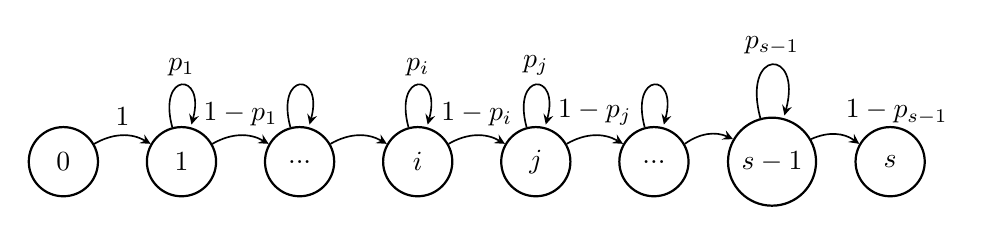
\begin{tikzpicture}[->, >=stealth, auto, semithick, node distance=1.5cm]
\tikzstyle{every state}=[fill=white,draw=black,thick,text=black,scale=1]
\node[state]    (A)                     {$0$};
\node[state]    (B)[right of=A]   {$1$};
\node[state]    (x)[right of=B]   {$...$};
\node[state]    (i)[right of=x]   {$i$};
\node[state]    (j)[right of=i]   {$j$};
\node[state]    (y)[right of=j]   {$...$};
\node[state]    (C)[right of=y]   {$s-1$};
\node[state]    (D)[right of=C]   {$s$};
\path
(A) edge[bend left]     node{$1$}     (B)
(B) edge[bend left]     node{$1-p_1$}     (x)
    edge[loop above]    node{$p_1$}       (B)
(x) edge[bend left]     node{}     (i)
    edge[loop above]    node{}       (x)
(i) edge[bend left]     node{$1-p_i$}     (j)
    edge[loop above]    node{$p_i$}       (i)
(j) edge[bend left]     node{$1-p_j$}     (y)
    edge[loop above]    node{$p_j$}       (j)
(y) edge[bend left]     node{}     (C)
    edge[loop above]    node{}       (y)
(C) edge[bend left]     node{$1-p_{s-1}$}   (D)
    edge[loop above]    node{$p_{s-1}$}     (D);
\end{tikzpicture}
\caption{Access Markov Chain, with $p_i=\frac{i}{n}$} \label{fig:AMC}
\end{figure} 
\begin{figure}

\[
\begin{bmatrix}
         0 & 1      &        &            &         &\text{\huge0}        \\
         0 & p_1    & 1-p_1  &            &         &        \\
          &        & p_2    & 1- p_2     &         &        \\
          &        &        & 1- p_{3} & p_{3} &        \\
          &        &        &            & p_4     & 1-p_4  \\
          &\text{\huge0}        &        &            &        & 1
\end{bmatrix}
\]

\caption{Corresponding Transition Matrix $P$, for $s=5$} \label{fig:ATM}
\end{figure}
The transition matrix $P$ represents the $s$ transient state, in which the stash is not completely filled, and the absorption state in which the stash is full.
Thus, $P$ can be decomposed in 4 submatrices: the square submatrix $Q_s$ representing all the transcient state, the column matrix R with the probabilities of transitioning to the absorbing state, the null row matrix and the absorption matrix.
\[
\begin{bmatrix}
   Q_s & R \\
   0_{1\times s}   & I_1 \\
\end{bmatrix}
\]
To find the average number of steps from one state to the absorbing one, we have solve the following equation, each row corresponding to the average number of steps from the corresponding state (the stashed filled with some records) to the state where the stash is full.
\begin{align*}
 t &= \left (\sum_{k=0}^{\infty} {Q_s}^k \right ) 1 \\
   &= (I_s -Q_s )^{-1} 1
\end{align*}
This equation has a solution since $M=I_s -Q_s$ have independant rows and thus an inverse that we call $N$.
By calculus we find that,
\begin{align*}
 n_{i,j} &= 0 &\text{ if } i>j,\\ 
 n_{i,j} &= \frac{1}{m_{i,i}} &\text{ if } i=j,\\
 n_{i,j} &= - n_{i+1,j } \cdot \frac{m_{i,i+1}}{m_{i,i}} &\text{ if } i<j 
\end{align*}
which can be simplified by
\begin{align*}
 n_{i,j} &= 0 &\text{ if } i>j,\\ 
 n_{i,j} &= \frac{1}{m_{j,j}} \prod_{k=1}^{j-1} \left ( - \frac{m_{i,k+1}}{m_{k,k}}\right ) &\text{ if } i\leq j
\end{align*}
We only want to calculate the first solution $S_1$ from the equation.
\begin{align*}
 S_1 &= \sum_{j=0}^{s-1} \frac{1}{m_{j,j}} \prod_{k=1}^{j-1} \left ( - \frac{m_{i,k+1}}{m_{k,k}}\right ) \\
     &= \sum_{j=1}^{s-1} \frac{1}{m_{j,j}} \text{ as } m_{i,k+1}= -m_{k,k} \\
     &= \sum_{j=0}^{s-1} \frac{1}{1-\frac{j}{n}}\\
     &= \sum_{j=0}^{s-1} \frac{n}{n-j}\\
     &= \sum_{j=0}^{s-1} \left (1 + \frac{j}{n-j} \right ) \\
     &= s + \sum_{j=0}^{s-1} \frac{j}{n-j} \\   
\end{align*}
As $s$ steps are required to fill the stash, we thus find the following inequality for the number of fake access $f$:
$$ \frac{s \cdot (s+1)}{2 \cdot n} < f < \frac{s \cdot (s+1)}{2 \cdot (n+1-s)} $$


\end{proof}

\end{document}